%avoid page number on blank pages when cleared
\thispagestyle{empty}
\cleardoublepage
\chapter{Theoretical Framework}
\label{sec:dev}
\section{Endrov}
\label{sec:endrov}

\emph{Endrov} is an open source plugin architecture aimed for image analysis and data processing.
Being based on \emph{Java}, it is portable and can both be run locally and as an applet, as mentioned
in \cite{web:endrov}. It grew out of the need for advanced open source software 
that can cope complex spatio-temporal image data, mainly obtained from microscopes in 
biological research. \emph{Endrov} aims to improve the features of the standard 
open source image analysis program, \emph{ImageJ}, by providing a more modern design.\\
The main issues with ImageJ are that it does not support metadata, there is no real support of 5D, 
the plugin architecture is messy, views cannot easily be extended and the batch 
process is difficult, as pointed out in \cite{web:endrovhome}.
Other problems that inspired the creation of \emph{Endrov} were: the lack of a standardize
image format and the difficulty to store complex data in the existing open formats.
The development group created the OST format in order
to handle the large image sets. OST is now a tree based object file format and it can store any 
type of data, but is optimized for images. 
Reading and writing single image panes is fast 
and there is no need to read everything into memory, \cite{web:endrovhome}.\\

Endrov is both a library and an imaging program. The design has made strong emphasis on 
separating GUI code from data types, filters and other data processing plug-ins. 
The idea is that the program can be used for most daily use or prototyping, and for 
bigger batch processing or integration, \cite{web:endrov}.\\

\emph{Endrov} was developed at the \emph{TBU Group, Karolinska Institute} and was officially released 
on 17 June 2009, under BSD license.



\section{Thresholding}
\label{sec:thresholding}

Thresholding is a process of image segmentation that can be used to create
binary images from gray-scale images. A binary image is a type of discrete image in
 which every pixel has assigned one of two possible values (typically 
$1$ or $0$) depending on whether the pixel belongs
to the foreground or to the background of the original image.

As stated on \cite{web:thresholding}, during the thresholding process individual 
pixels in an image are marked as ``object'' pixels if 
their value is greater than some threshold value (assuming an object to be brighter than the 
background) and as ``background'' pixels otherwise. This convention is known as \emph{threshold above}. 
Variants include \emph{threshold below}, which is opposite of threshold above; \emph{threshold inside}, where a 
pixel is labeled "object" if its value is between two thresholds; and \emph{threshold outside}, which is 
the opposite of \emph{threshold inside} \cite{shapiro}.

In image processing applications where the study is focused on particular objects contained
in an image, thresholding becomes a simple tool to separate these objects from
the background, but not always accurate. Commonly, the gray levels belonging to the object are substantially
different from the gray levels of the background pixels. In \cite[p.146]{thres} many thresholding
applications in image processing are mentioned such as: document image analysis, where the goal
is to extract printed characters, logos, graphical content, or musical scores; map processing
where lines, legends and characters are to be found; scene processing, where a target is to
be detected; and quality inspection of materials, where defective parts must be delineated,
among many others. \\

The key parameter in the thresholding process is the thresholding value (or values for
\emph{threshold inside approach}). The value can be automatically computed, what is called
\emph{automatic thresholding}, as well as set or tuned through user input.\\
According to the information they are exploiting, the different thresholding methods can be 
categorized. In \cite[p.147]{thres}, Sezgin and Sankur categorize the thresholding methods in
six groups:
\begin{itemize}
\item Histogram shape-based methods: the peaks, valleys and curvatures of the smoothed
histogram are analyzed
\item Clustering-based methods: gray-level samples are clustered in two parts as
background and foreground, or modeled as a mixture of two Gaussians.
\item Entropy-based methods: algorithms that use the entropy of the foreground 
and background regions, the cross-entropy between the original and the binary image, 
etc.
\item Spatial methods: use higher-order probability distribution and/or 
correlation between pixels
\item Local methods: adapt the threshold value on each pixel
to the local image characteristics.
\end{itemize}

In fig. \ref{fig:thres1}, two images are shown that correspond to a gray-scale image
and binary image obtained by thresholding.

\begin{figure}[h t b p ! H]
  \centering
  \subfloat[Gray-scale Image]{\label{fig:threso}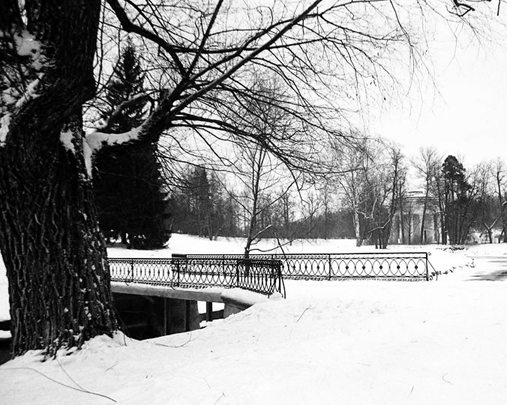
\includegraphics[width=0.45\textwidth]{thres/winter_o}}
\qquad
  \subfloat[Binary image obtained through thresholding]{\label{fig:thres1}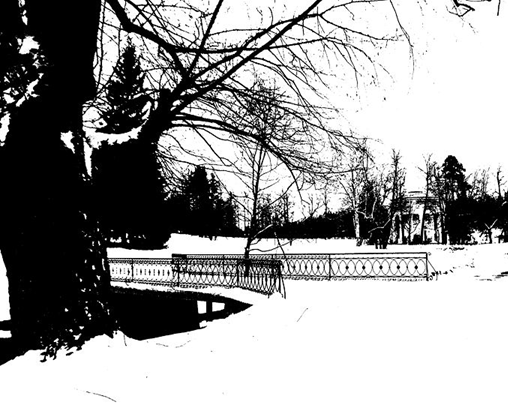
\includegraphics[width=0.45\textwidth]{thres/winter_thres}}
  \caption[Gray-scale Image before and after a thresholding effect is applied]{Gray-scale Image before and after a thresholding effect is applied. Images taken from \cite{web:thresholding}}
  \label{fig:thres1}
\end{figure}

\section{Distance Transform}
\label{sec:dt}

A distance transform or distance map is a representation of a digital image
in which each pixel has a value corresponding to the distance to the 
nearest non-object pixel. It is calculated from a digital binary image, 
consisting in object and non-object pixels. The object 
pixels can be considered as foreground and the non-object pixels as
background. The obtained image is then a sort of gray-scale representation
of the foreground pixels in the binary image.\\
The pixel mapping depends mainly on the distance metric, which is the 
measurement method of distance between image pixels. Different metrics have been 
studied to find distance maps such as 
\emph{City Block or Manhattan},
\emph{Chessboard}, \emph{Euclidean}, \emph{Chamfer 3-4}, \emph{Octagonal}, among
others.\cite[p.363]{dtresearch}. There exist great amounts of
distance metrics of other kinds that are useful for different purposes.
These are commonly derived from the previous.
Fig. \ref{fig:dtexamples} shows the images obtained by applying different distance metrics.

\begin{figure}[h t b p ! H]
 \centering
   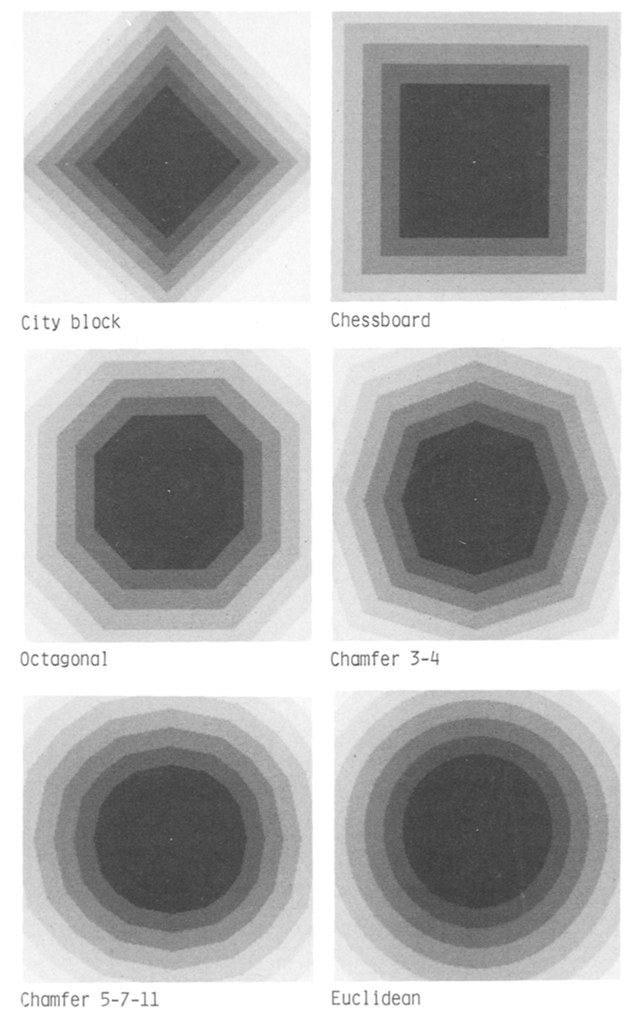
\includegraphics[scale=0.4]{dt/dtref}
 \caption[The distances from a point for the six distance transformations]{The distances from a point for the six distance transformations.
 The lighter the color the larger the distance \cite[p.365]{dtresearch}}
 \label{fig:dtexamples}
\end{figure}

As stated in \cite{dtresearch2} 
distance transforms play a central role in the comparison of binary images, 
particularly for images resulting from local feature detection techniques such 
as edge or corner detection. For example, both the Chamfer
and Hausdorff matching approaches make use of distance transforms in comparing binary images. 
Distance maps can also be interpreted as landscapes of islands 
where the label of every pixel indicates the height of the region. This allows
the detection of ridges and peaks which is a straightforward way to find the
skeleton of an object.\cite[237]{ridgedt}. The nature of distance transforms
in which the objects are represented as contour layers of different depth
makes them also a useful tool for edge analysis and to improve efficiency of 
morphology algorithms such as \emph{Thinning} and \emph{Thickening}.\\

\section{Skeletonization}
\label{sec:skeletonization}

A skeleton is a compact and simple representation of an object that consists of a thin
version of it that is equidistant to its boundaries and preserves many of
the topological and geometrical characteristics of the original image, as explained in
\cite{wikipedia:skeleton,ssm,augmented}. Usually the skeleton is defined as the centers
of maximal discs contained in the original image, \cite{ssm,augmented}.
Regardless of the definition that is adopted, if the skeleton points are attributed with their distances
to the original boundary of the object, the skeleton can be used to exactly 
reconstruct the original shape. Figure \ref{fig:genskeleton} shows a skeleton calculated
from a horse shape and the original binary image.\\

\begin{figure}[h t b p ! H]
  \centering
  \subfloat[Binary Image]{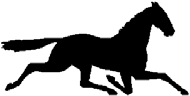
\includegraphics[scale=0.8]{skeleton/horsebinary}}
\qquad
  \subfloat[Image Skeleton]{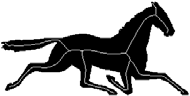
\includegraphics[scale=0.8]{skeleton/horseskeleton}}
  \caption[Horse binary shape and skeleton]{Horse binary shape and skeleton. 
Images taken from \cite{ssm}}
  \label{fig:genskeleton}
\end{figure}


Depending on the way they are produced, skeletons can be categorized in different types.
Telea et al describe three types in \cite{augmented}, such as: \emph{Morphological Thinning},
\emph{Geometric Methods} and \emph{Distance transform}. The \emph{Morphological Thinning} methods iteratively peel off (or reduce) the boundary, layer by layer, identifying
points whose removal does not affect the object's topology. These are usually 
straightforward and normally require intricate heuristics to ensure the skeletal
connectivity, as mentioned in \cite{augmented}. Two fast parallel approaches that
ensure connectivity using the \emph{Morphological thinning} method are described
in \cite{onepass} and \cite{thinning}.\\
The \emph{Geometric Methods} compute the Voronoi diagram of a discrete polyline-like
sampling of the boundary. A Voronoi diagram is the boundary's medial axis. ``Such 
methods produce an accurate connected skeleton, but are fairly complex to implement,
require a robust boundary discretization, and are computationally expensive''
\cite[p.251]{augmented}.\\
Another method computes \emph{the distance transform}
(see Sec. \ref{sec:dt}) of the objects boundary. The common approach consists in
finding the ridge points and connecting them \cite{maxima,euclideancentre,ridgedt}.
 Usually they can ensure the accurate localization of skeleton points 
but neither connectivity nor completeness.\\

Skeletons are important for object representation and recognition in different areas,
such as: computer vision, image analysis, and digital image processing, 
including optical character recognition, fingerprint recognition, visual inspection,
pattern recognition, binary image compression, and protein folding \cite{skprotein}.


\section{Shape Matching}
\label{sec:shapefitting}

Shape matching is a central problem in visual information systems,
computer vision, pattern recognition and robotics \cite{matchingbook}. 
It consists of identifying the area or contour of a specific
shape or class of shapes in an image, and plays a fundamental
role in content extraction from images and content-based image
retrieval. In \cite{matching2}, Veltkamp explains that shape 
matching deals with transforming a shape and measuring the 
resemblance with another one, using some similarity measure, that 
normally correspond to the notion of distance between shapes.\\
The concept of shape is abstract, but most approaches in 
shape matching represent a shape as a geometrical object.
This can be both a set of points, curves, surfaces, solids etc.
and a geometrical pattern modulo some transformation group,
in particular similarity transformations (translation, rotation 
and scaling), as is stated in \cite{matching2}. Usually a
geometrical pattern of a shape called shape descriptor
is used to represent the class of the matching object. There are
different types of shape descriptors depending on the information
they supply and the nature of the problem (see Sec.\ref{sec:shapedesc}) \\

There are different studied approaches to the shape matching 
problem. The emphasis on this section will be on the Computational
Geometry based approaches for shape matching, since is the most related with
the approach followed in this thesis work. Computational
Geometry studies algorithms that can be declared in terms of 
geometry.\\

In \cite{matchingbook} Veltkamp and Hagedoorn mention different 
approaches of shape matching such as: tree pruning, the
generalized Hough transform or pose clustering, geometric hashing,
the alignment method, statistics, deformable templates, relaxation
labeling, Fourier descriptors, wavelet transform, curvature
scale space and neural networks.
They also categorize the matching techniques in two main groups:
\emph{global image transforms} and \emph{global objects methods}.
The \emph{global image transform} group refers to the techniques that
``transform the image from color information in the spatial
domain to color variation in the frequency domain''. 
These approaches do not represent the shape explicitly for 
matching, instead they represent color or intensity transitions 
in the image. This makes it impossible to measure the difference of 
two images in terms of shape as well as to match a shape with a 
specific part of an image.\\
On the other hand the \emph{global object methods} work with a complete
object area or contour and can analyze specific areas in the 
image instead of requiring processing the whole image as in 
the global image transforms. In order to perform a proper
matching, the objects in the image have to be completely and
clearly segmented. Some of these methods are: \emph{moments}, where an
object is described as a set of moments, \emph{modal matching},
where the boundary is used instead of the area and is described 
with Fourier descriptors and \emph{curvature scale space}, where a
scale space and parameterized representation of the contour of the 
objects is used.\\

Veltkamp describes in \cite{matching2} various forms in
which shape matching is studied, given two shape patterns
and a dissimilarity measure. These are:

\begin{itemize}
\item \textbf{Computation Problem: }Compute the dissimilarity
  between the two patterns
\item \textbf{Decision Problem: }
  \begin{itemize}
  \item  For a given threshold, decide
  whether the dissimilarity is smaller than the threshold.
  \item For a given threshold, decide
    whether there exists a transformation such that the
    dissimilarity between the transformed pattern and the other 
    pattern is smaller than the threshold
  \end{itemize}
 
\item \textbf{Optimization Problem: }Find the transformation
that minimizes the dissimilarity between the transformed
pattern and the other pattern.
\end{itemize}

A well studied optimization approach for shape matching is
Active Contour Models (\emph{Snakes}),  which inspired much 
of the shape fitting approach of this work 
(see Sec \ref{sec:metfit}). In \cite{snakes} a snake is defined 
as an energy-minimizing spline guided by external constraint
forces and influenced by image forces that pull it toward 
features such as lines and edges. The \emph{snakes} are said to
be active contour models because they lock onto nearby edges,
localizing them accurately.\\
The \emph{snakes} model is defined as a controlled continuous spline that is bound
by internal and external image forces, called energies. The external energy models how well
the deformed model matches the data. The internal energy models
the objects resistance to be pushed by the external force into directions not coherent
with the prior knowledge \cite{deformable}. In this case, the internal energy  imposes 
a ``piecewise smoothness constraint'' \cite{snakes}. This means that a contour is
pushed to an image feature by the external force while the contour itself exhibits resistance
to be deformed into a non-smooth curve. As explained in \cite{deformable} the image forces push the snake toward
salient image features like line, edges and subjective contours, while the external constraint forces
are responsible for putting the snake near the desired local minimum.\\

Given these definitions, let $M$ be the model and $D$ a data set, 
the total energy $E$ can be defined as:

$$E(M) = E_{ext}(M,D) + E_{int}(M)$$

where $E_{ext}$ is the external energy function and $E_{int}$ the 
internal energy function. 
Having this, the optimization algorithm consists of minimizing the objective
function until the best solution is found.


\section{Shape descriptor}
\label{sec:shapedesc}

A shape descriptor is a structured abstraction of a class
of shapes that describes them in geometrical terms.
Shape descriptors can have either fixed or variable
geometrical shapes. Variable descriptors depend on the different values assigned to its
parameters, different shapes are generated but still belong to the same type or class of shapes.
Shape models have been used widely to achieve robust interpretation of complex
images \cite{wormparam}. They allow image evidence to be organized into plausible interpretations
which can then be verified.\\

Latecki et al \cite{shapenonrigid}, divide shape descriptors into three
main categories: 
\begin{itemize}
\item \textbf{Contour based descriptors: }The contour of a given object is 
mapped to some representation from which a shape descriptor is derived
\item \textbf{Image based descriptors: }The computation of a shape descriptor
is based on summing up pixel values in a digital image containing the silhouette
of a given object; the shape descriptor is a vector of a certain number of
parameters derived this way
\item \textbf{Skeleton based descriptors: }After a skeleton is computed, it is
mapped to a tree structure that forms the shape descriptor; the shape similarity
is computed by some tree-matching algorithm 
\end{itemize}

Considering that basically shape descriptors are ``attempts to quantify shape in 
ways that agree with human intuition''\cite[p.1]{desclecture}, any kind of 
geometrical interpretation that covers the contents or properties that want 
to be described on a shape, can be used as a shape descriptor.
In \cite{desclecture} region-based shape descriptors. These are such descriptors
that attempt to describe a shape based on the geometrical and numerical properties
of the region of the shape. Some simple descriptors are mentioned such as:
area, perimeter, (Non-)Compactness or (Non-)Circularity, Eccentricity, Elongation,
Rectangularity and Orientation. Any combination of these properties of a shape are
useful to describe them in a basic and general way.
Other more complex properties are mentioned to improve the accuracy of the 
descriptor: \emph{convex hull}, \emph{extremal points}, \emph{profiles}, 
\emph{ moments} and \emph{profile moments}. \emph{Convex hull or bays} 
describes the shape by measuring the number or size of concavities in the 
shape. \emph{Extremal points} is based on finding the points that
are at the extreme of the shape. This can be a simple representation as the 
\emph{bounding box} or a more powerful one as it is finding the eight extremal
points defined by: top left, top right, left top, left bottom, bottom right,
bottom left, right top and right bottom. The \emph{Profiles} shape descriptor 
is based on the number of pixels that the shape has in a given direction:
 either vertical, horizontal or diagonal. \emph{Moments} refer to the
 calculation of \emph{moment} statistical properties and 
\emph{profile moments}, or a combination of the last two.\\
In \cite{web:wikishape}, shape descriptors are classified by their
invariance with respect to the transformations allowed in the associated
shape definition. The main classes are descriptors invariant with respect 
to congruence and descriptors invariant with respect to isometry. 
The congruence class
comprehends identical shape descriptors for congruent shapes 
(shapes obtained from
translation, rotation or mirroring). The intrinsic shape descriptor refer
to those that do not change with different isometric embedding of the shape,
and thus can be applied accurately to deformable objects.

Depending on the properties that are controlled and measured, the descriptor
may or may not allow reconstructing a shape of the class. In \cite{wormparam}, 
a trainable method of shape representation is described which can
automatically capture the invariant properties of a class of shapes and 
provide a compact parametric description of variability. The method was
applied on worms, obtaining a shape descriptor that reconstruct different
bending worm shapes by modifying the values of the parameters.\\

\section{Splines}
\label{sec:splines}

The term spline, as it is used in this work, refers to a piecewise polynomial curve. Splines
are widely used in computer science subfields because of the simplicity of their constructions,
their ease and accuracy of evaluation, and their capacity to approximate complex shapes
through curve fitting and interactive curve design, as mentioned in \cite{web:splines}.
The continuous signal representation is particularly apposite for 
problems such as: edge detection, surface fitting and multi-resolution
techniques. It is useful for many other problems in computer
vision such as: optical flow, surface reconstruction, the recovery
of lightness and color, shape from shading and stereo matching,
\cite[821]{splinespap}.

Special types of splines receive different names, depending on different conditions.\\
A commonly used type of spline in object recognition is the Hermite spline. This is a third-degree spline, expressed using Hermite polynomials to represent each of the 
individual polynomial pieces. 
Several methods have been invented to fit such splines to given data points such
as \emph{Cardinal Splines, Catmull-Rom splines, Kochanek-Bartels splines}. They allow constructing smooth curves that go through every point in a given data set. Thus, \emph{e.g.} 
given a series of points belonging to the contour of an object, a smooth shape can be 
calculated that models the shape of the defined object.  
Such as B-splines, Hermit splines have a number of advantages for image processing, as
mentioned in \cite{splinespap}.
First, they are usually smooth and well behaved, therefore they do not tend to oscillate
as higher order polynomials do. Second, the juxtaposition of local polynomial approximations
may produce strong discontinuities in the connecting regions. B-spline
surfaces, by contrast, are continuous everywhere. 
Finally, they can be evaluated efficiently.
